\documentclass[10pt]{article}
\usepackage[polish]{babel}
\usepackage[utf8]{inputenc}
\usepackage[T1]{fontenc}
\usepackage{amsmath}
\usepackage{amsfonts}
\usepackage{amssymb}
\usepackage[version=4]{mhchem}
\usepackage{stmaryrd}
\usepackage{graphicx}
\usepackage[export]{adjustbox}
\graphicspath{ {./images/} }

\title{III Konkurs Matematyczny St@ś XIV LO im. Stanisława Staszica 29 kwietnia 2003 roku }

\author{}
\date{}


\begin{document}
\maketitle
\section*{klasa VI}
Na rozwiqzanie poniższych zadań masz 90 minut. Kolejność rozuniqzwania tych zadań jest dowolna. Wszystkie zadania sa jednakowo punktowane. Maksymalna liczbę punktów może uzyskać jedynie pelne rozwiqzanie, z uzasadnieniem i odpowiedziq.\\
Używanie korektora i korzystanie z kalkulatora jest niedozwolone.

\section*{Zadanie 1.}
Na stole leżą 2003 monety. Jaś w jednym ruchu może wziąć dokładnie 3, 15 lub 54 monet.\\
Czy Jaś, wykonując wiele takich ruchów, może wziąć wszystkie monety ze stołu?

\section*{Zadanie 2.}
Podaj przykład takiej liczby, której kwadrat jest większy od 124, a sześcian jest mniejszy od 124.

\section*{Zadanie 3.}
Oblicz: \(\quad \frac{1}{2}+\frac{5}{6}-\frac{1}{3}+\frac{7}{10}-\frac{1}{5}+\frac{9}{14}-\frac{1}{7}+\frac{11}{18}-\frac{1}{9}+\frac{13}{22}-\frac{1}{11}+\frac{15}{26}-\frac{1}{13}\).

\section*{Zadanie 4.}
Z jednego wierzchołka sześcianu poprowadzono przekątre dwóch sąsiednich ścian.\\
Oblicz miarę kąta między tymi przekątnymi.

\section*{Zadanie 5.}
Pięciokąt \(A B C D E\) jest foremny, a trójkąt \(A B F\) jest równoboczny. Każdy kąt wewnętrzny pięciokąta foremnego ma \(108^{\circ}\). Oblicz miarę kąta \(B F C\).\\
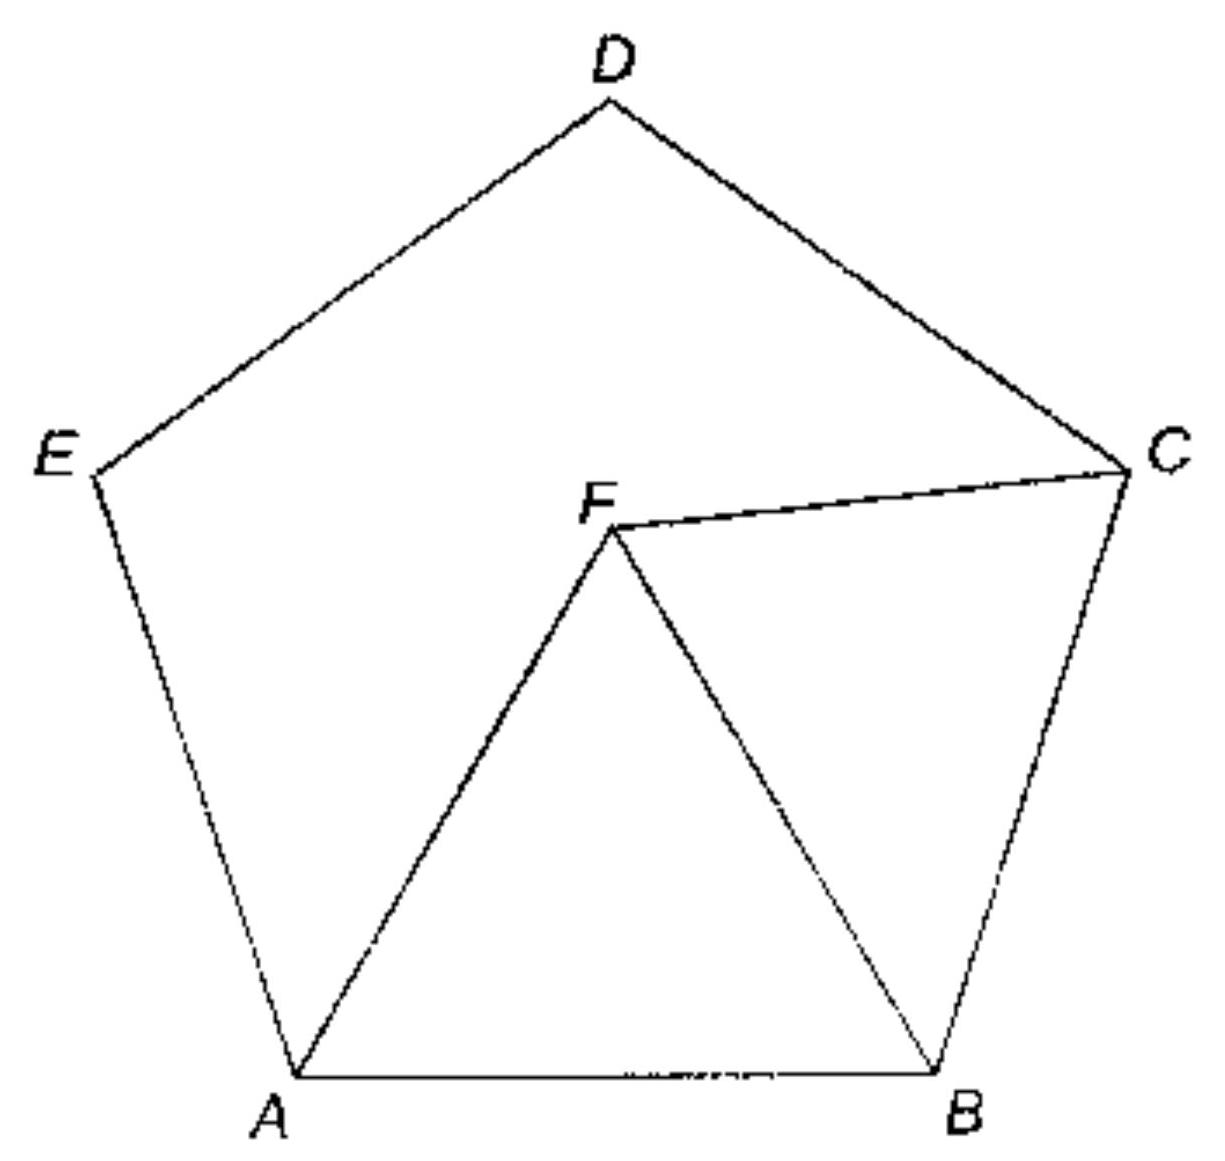
\includegraphics[max width=\textwidth, center]{2024_11_21_463a1300a95b8e89e62eg-1}


\end{document}